%\documentclass[show notes]{beamer}       % print frame + notes

\documentclass[11pt,handout]{beamer}   % only notes
%\documentclass[aspectratio=169]{beamer}              % only frames
\usefonttheme[onlymath]{serif}
\definecolor{DarkGray}{HTML}{63656a}
\setbeamertemplate{note page}[plain]
\setbeamertemplate{navigation symbols}{}
\setbeamertemplate{footline}[text line]{%
  \hfill\strut{\scriptsize\sf\color{DarkGray}\today}\hfill\strut{%
        \scriptsize\sf\color{DarkGray}%
        \quad\insertframenumber/\inserttotalframenumber
    }%
}

\usepackage{amsfonts}


\beamertemplatenavigationsymbolsempty


\title[Your Short Title]{Nonlinear Control Systems}
\subtitle{Lsn 4: Advanced Stability Theory}
\author{I. Weintraub, Dr. Cobb, \& Capt. Hess}
\institute{Air Force Institute of Technology}
\date{\today}

\begin{document}

\begin{frame}
  \titlepage
\end{frame}


\begin{frame}
\frametitle{Advanced Stability Theory}
\textbf{Concepts Concerning Stability}
\begin{itemize}
\item Concepts of stability for non-autonomous systems
\item Lyapunov analysis of non-autonomous systems
\item Instability theorems
%\item Existence of Lyapunov functions
\item Lyapunov Analysis using Barbalat's Lemma
%\item Positive linear systems
%\item The passivity formalism
%\item Absolute Stability
%\item Establishing boundedness signals
%\item Existence and unicity solutions
\end{itemize}

\begin{table}
\centering
    \begin{tabular}{l  c}
    \hline
     & Topic \\ \hline
    $\checkmark$ Week 1 & Introduction and Math Review\\
    $\checkmark$ Week 1-2 & Phase Plane Analysis\\
    Week 2-4 & Fundamentals of Lyapunov Theory\\
    Week 4   & Advanced Stability Theory\\
    Week 4-5 & Describing Functions \\
    Week 5-7 & Feedback Linearizion \\ 
    Week 8-9 & Sliding Mode Control \\
    Week 10  & Adaptive Control \\\hline
    \end{tabular}
\end{table}

\end{frame}


\begin{frame}
\frametitle{Concepts of Stability for Non-Autonomous Systems}
\small
Due to the dependence of non-autonomous system behavior on initial time, $t_0$, definitions include $t_0$ explicitly.\\
\vspace{6pt}
\textbf{Non-Autonomous System}
\begin{equation*}
\dot{\mathbf{x}} = \mathbf{f}(\mathbf{x},t)
\end{equation*}
Has an equilibrium point $\mathbf{x}^*$:
\begin{equation*}
\mathbf{f}(\mathbf{x}^*,t) = 0 \quad \forall  \; t \geq t_0
\end{equation*}
\textbf{Definition:} An equilibrium point $\mathbf{0}$ is \underline{stable} at $t_0$ if for any $R>0$ there exists a positive scalar $r(R,t_0)$ such that:
\begin{equation*}
||\mathbf{x}(t_0)|| < r \Rightarrow ||\mathbf{x}(t)||<R \quad \forall \; t \geq t_0
\end{equation*}
Otherwise the point $\mathbf{0}$ is unstable.\\
\vspace{6pt}
We can keep the state in a ball of arb. small radius $R$ by starting the state trajectory in a ball of sufficiently small radius $r$.
\end{frame}

\begin{frame}
\frametitle{Concepts of Stability for Non-Autonomous Systems}
\small
\textbf{Definition:} The equilibrium point $\mathbf{0}$ is \underline{asymptotically stable} at a time $t_0$ if:
\begin{enumerate}
\item It is stable
\item $\exists \; r(t_0) > 0$ s.t. $||\mathbf{x}(t_0)||<r(t_0) \Rightarrow ||\mathbf{x}(t)|| \rightarrow \mathbf{0}$ as $t \rightarrow \infty$
\end{enumerate}
Requires that there exists an attractive region for every initial time $t_0$.\\
\vspace{6pt}
\textbf{Definition:} The equilibrium $\mathbf{0}$ is \underline{exponentially stable} if there exists two positive numbers $\alpha \; \& \; \lambda$ s.t. for sufficiently small $\mathbf{x}(t_0)$:
\begin{equation*}
|| \mathbf{x} || \leq \alpha || \mathbf{x} (t) || e^{- \lambda(t - t_0)} \quad \forall \; t \geq t_0
\end{equation*}
\textbf{Definition:} The equilibrium point $\mathbf{0}$ is \underline{globally asymptotically stable} if $\forall \mathbf{x}(t_0)$:
\begin{equation*}
\mathbf{x}(t) \rightarrow \mathbf{0} \; \text{as} \; t \rightarrow \infty
\end{equation*}
\end{frame}

\begin{frame}
\frametitle{Concepts of Stability for Non-Autonomous Systems}
\small
\textbf{Example:} $\mathbf{\dot{x}}(t) = -a(t)\mathbf{x}(t)$
The solution to this first order differential equation is: $\mathbf{x}(t) = \mathbf{x}(t_0) \exp \left[  -\int_{t_0}^{t} a(r) dr \right]$\\
\begin{itemize}
\item The system is \underline{stable} if $a(t) \geq 0 \; \forall \; t\geq t_0$
\item The system is \underline{asymptotically stable} if $\int_{0}^{\infty} a(r) dr = +\infty$
\item The system is \underline{exponentially stable} if there exists $T>0$ s.t. $\forall \; t \; \geq 0$ , $\int_{t}^{t+T} a(r) dr \geq \gamma $ where $\gamma = \text{const.} > 0$. 
\end{itemize}
Examples:
\begin{itemize}
\item ${\dot{x}} = - \frac{x}{(1+t)^2}$ is stable but not asymptotically stable
\item ${\dot{x}} = - \frac{x}{(1+t)}$ is asymptotically stable
\item ${\dot{x}} = - t x$ is exponentially stable
\end{itemize}
\end{frame}

\begin{frame}
\frametitle{Concepts of Stability for Non-Autonomous Systems}
\small
\textbf{Uniformity:} ``In practice it is usually desirable for the system to have certain uniformity in its behavior regardless of when the operation starts''- Slotine. Because the behavior of autonomous systems is independent of the initial time, all the stability properties of an autonomous system are uniform.\\
\vspace{6pt}
\textbf{Definition:} the equilibrium point $\mathbf{0}$ is \underline{locally uniformly stable} if the scalar $r$ chosen independent of $t_0$:
\begin{equation*}
\forall t \geq t_0 \; , \; ||\mathbf{x}(t_0)|| < r \Rightarrow ||\mathbf{x}(t)|| < R \quad  \text{i.e. if:} \; r = r(R)
\end{equation*}
\textbf{Definition:} The equilibrium point at the origin is locally \underline{uniformly asymptotically stable} if:
\begin{itemize}
\item It is uniformly stable
\item There exists a ball of attraction $\mathbf{B_{R_0}}$, whose radius is independent of $t_0$, such that any system trajectory with initial states in $\mathbf{B_{R_0}}$ converge to $\mathbf{0}$ uniformly in $t_0$.
\end{itemize}
\end{frame}

\begin{frame}
\frametitle{Concepts of Stability for Non-Autonomous Systems}
\small
\textbf{Uniform Convergence}: For all $R_1$ and $R_2$ satisfying $0<R_2<R_1\leq R_0 \; \exists \; T(R_1,R_2) >0$ s.t. $\forall t_0 \geq 0$.
\begin{equation*}
||\mathbf{x}(t_0)|| < R_1 \Rightarrow ||\mathbf{x}(t)|| < R_2 \quad \forall t \geq t_0 + T(R_1,R_2)
\end{equation*}
The state trajectory starting from within a ball $\mathbf{B}_{R_1}$ will converge into a smaller ball $\mathbf{B}_{R_2}$ after a time period $T$ which is independent of $t_0$.\\
\vspace{6pt}
Exp. Stability $\Rightarrow$ Unif. Asymp. Stability $\Rightarrow$ Asymp. Stability\\
\vspace{6pt}
\textbf{Example:} $\dot{x} = - \frac{x}{1+t}$ has general solution:\\
\begin{equation*}
x(t) = \frac{1 + t_0}{1 + t} x(t_0)
\end{equation*}
Note that this first order system is asymptotically stable, but not uniformly since larger $t_0$ requires longer time to get close to the origin.\\
\vspace{6pt}
\underline{Global Uniformly Asymptotic Stability} replaces ball of attraction $\mathbf{B}_{R_0}$ by the entire state space.
\end{frame}

\begin{frame}
\frametitle{Lyapunov Analysis of Non-Autonomous Systems}
\small
\textbf{Lyapunov's Direct Method of Non-Autonomous Systems}\\
\vspace{3pt}
A scalar time-varying function $V(\mathbf{x},t)$ is \underline{locally positive definite} if $V( \mathbf{0},t) =0$ and there exists a time-invariant positive definite function $V_0(\mathbf{x})$ such that:
\begin{equation*}
\forall \; t \geq t_0 \quad V( \mathbf{x},t) \geq V_0(\mathbf{x})
\end{equation*}
Therefore a time-variant function is locally positive definite if it dominates a time-invariant locally positive definite function.\\
\vspace{6pt}
\textbf{Definition:} A scalar function  $V(\mathbf{x},t)$ is \underline {decrescent} if $V(\mathbf{0},t) = 0$ and if there exists a time-invariant positive definite function $V_1(\mathbf{x})$ such that:
\begin{equation*}
\forall \; t \geq 0 \;,\; V(\mathbf{x},t) \leq V_1(\mathbf{x})
\end{equation*}
A function $V(\mathbf{x},t)$ is decrescent if it is dominated by a time-invariant positive definition function.
\end{frame}

\begin{frame}
\frametitle{Lyapunov Analysis of Non-Autonomous Systems}
\small
\textbf{Example:} $V(\mathbf{x},t) = ( 1 + \sin ^2 t)(x_1^2 + x_2^2)$\\
This is a time-varying positive definite function because it dominates the function: $V_0(\mathbf{x}) = x_1^2 + x_2^2$.  This function is also decrescent because it is dominated by the function $V_1(\mathbf{x}) = 2(x_1^2 + x_2^2)$.\\
\vspace{6pt}
\textbf{Chain Rule for Time Varying Functions:}
\begin{equation*}
\frac{d V}{d t} = \frac{\partial V}{\partial t} + \frac{\partial V}{\partial \mathbf{x}}\dot{\mathbf{x}} = \frac{\partial V}{\partial t} + \frac{\partial V}{\partial \mathbf{x}} f(\mathbf{x},t)
\end{equation*}
\textbf{Lyapunov Thm. for Non-Autonomous Systems}\\
If in a ball $\mathbf{B}_{R_0}$ around the equilibrium point $\mathbf{0}$, there exists a scalar function $V(\mathbf{x},t)$ with continuous partial derivatives such that:
\begin{enumerate}
\item $V$ is positive definite
\item $\dot{V}$ is negative semi-definite
\end{enumerate}
Then the equilibrium point $\mathbf{0}$ is stable in the sense of Lyapunov
\end{frame}

\begin{frame}
\frametitle{Lyapunov Analysis of Non-Autonomous Systems}
\footnotesize
\textbf{Uniform stability and uniform asymptotic stability}\\
If in a ball $\mathbf{B}_{R_0}$ around the equilibrium point $\mathbf{0}$, there exists a scalar function $V(\mathbf{x},t)$ with continuous partial derivatives such that:
\begin{enumerate}
\item $V$ is positive definite
\item $\dot{V}$ is negative semi-definite
\item $V$ is decrescent
\end{enumerate}
the origin is \underline{uniformly stable}.\\
\vspace{6pt}
\textbf{Further:}\\
If $\dot{V} < 0$ then the equilibrium point is uniformly asymptotically stable.\\
\vspace{6pt}
\textbf{Global uniform asymptotic stability}\\
If in the \underline{whole state space} there exists a scalar function $V(\mathbf{x},t)$ with continuous partial derivatives such that:
\begin{enumerate}
\item $V$ is positive definite
\item $\dot{V}$ is negative semi-definite
\item $V$ is decrescent
\item $V(\mathbf{x},t)$ is radially unbounded
\end{enumerate}
the origin is \underline{globally uniformly asymptotically stable}.
\end{frame}

\begin{frame}
\frametitle{Lyapunov Analysis of Non-Autonomous Systems}
\small
\textbf{Example:}
\begin{equation*}
\begin{aligned}
\dot{x}_1 &= -x_1(t) - e^{-2t} x_2(t)\\
\dot{x}_2 &= -x_1(t) - x_2(t)
\end{aligned}
\end{equation*}
To determine the stability of the equilibrium point at $\mathbf{0}$ , let us choose the following scalar function: $V(\mathbf{x},t) = x_1^2 + (1+e^{-2 t} )x_2^2$. \\
\vspace{6pt}
This function is positive definite, because it dominates the time-invariant positive function $x_1^2 + x_2^2$. It is also decrescent because it is dominated by the time-invariant positive definite function $x_1^2 + 2x_2^2$. Furthermore:
\begin{equation*}
\dot{V}(\mathbf{x},t) = -2(x_1^2 - x_1 x_2 + x_2^2(1+2 e^{-2t}))
\end{equation*}
Shows that 
$\dot{V} \leq -2(x_1^2 - x_1 x_2 +x_2^2) = -(x_1 - x_2)^2 - x_1^2 - x_2^2$\\
\vspace{6pt}
Thus $\dot{V}$ is negative definite, and therefore, the point $\mathbf{0}$ is globally asymptotically stable.\\
\vspace{6pt}
\large
``Stability results for non-autonomous systems can be less intuitive than those for autonomous systems'' - Slotine\\
\begin{tiny}
Examples: Slotine (pp 111-113)
\end{tiny}
\end{frame}

\begin{frame}
\frametitle{Lyapunov Analysis of Non-Autonomous Systems}
\small
\textbf{Lyapunov Analysis of Linear Time-Varying Systems}\\
\vspace{6pt}
Consider the linear-time varying system:
\begin{equation*}
\mathbf{\dot{x}} = \mathbf{A}(t) \mathbf{x}
\end{equation*}
``Since LTI systems are asymptotically stable if their eigenvalues all have negative real parts, once might be tempted to conjecture that systems of the type, $\mathbf{\dot{x}} = \mathbf{A}(t)\mathbf{x}$, will be stable if at any time $t \geq 0 $ all eigenvalues of $\mathbf{A}(t)$ all have negative real parts...'' However, this is not sufficient for stability of time-varying linear systems.\\
\textbf{Example:}
\begin{equation*}
\frac{d}{dt}\begin{bmatrix}
x_1 \\ x_2
\end{bmatrix} = \begin{bmatrix}
-1 & e^{2t} \\ 0 & -1
\end{bmatrix} \begin{bmatrix}
x_1 \\ x_2
\end{bmatrix}
\end{equation*}
Solving:
\begin{equation*}
x_2 = x_2(0) e^{-t} \quad \dot{x}_1 + x_1 = x_2(0)e^t
\end{equation*}
$x_2(0) e^t$ tends to infinity and we can see that $x_1$ will grow and the system is unstable. Although the eigenvalues of $\mathbf{A}$ are both equal to $-1$ at all times.\\
\textbf{}
\end{frame}

\begin{frame}
\frametitle{Lyapunov Analysis of Non-Autonomous Systems}
\small
\textbf{Lyapunov Analysis of Linear Time-Varying Systems}\\
\vspace{6pt}
\textbf{Solution:} look at the eigenvalues of the symmetric matrix $\mathbf{P}(t) = \mathbf{A}(t) + \mathbf{A^T}(t)$.\\
\vspace{6pt}
The time varying system $\mathbf{\dot{x}} = \mathbf{A}(t) \mathbf{x}$ is asymptotically stable if the eigenvalues of the symmetric matrix $\mathbf{P}(t)$ remain strictly in the left-half complex plane.\\
\begin{equation*}
\exists \; \lambda > 0 , \forall \; i \; , \forall t \geq 0 , \lambda_i (\mathbf{A}(t) + \mathbf{A^T}(t)) \leq - \lambda
\end{equation*}
This can be readily shown using the Lyapunov function $V = \mathbf{x^T x}$ since:
\begin{equation*}
\dot{V} = \mathbf{x^T \dot{x}} + \mathbf{\dot{x}^T x} = \mathbf{x^T (A}(t)\mathbf{ + A^T}(t)\mathbf{) x} \leq -\lambda \mathbf{x^Tx} = - \lambda V
\end{equation*}
so that:
\begin{equation*}
\forall \; t \geq 0 , \quad   0 \leq \mathbf{x^Tx} = V(t) \leq V(0) e^{-\lambda t}
\end{equation*}
\end{frame}

\begin{frame}
\frametitle{Lyapunov Analysis of Non-Autonomous Systems}
\small
\textbf{Perturbed Linear Systems}\\
Consider: $\mathbf{\dot{x}} = (\mathbf{A_1 + A_2}(t))\mathbf{x}$\\
\begin{itemize}
\item $\mathbf{A}_1$ is const. with all eigenvalues in the L.H.P. (\textit{Hurwitz}).
\item $\mathbf{A}_2(t) \rightarrow 0 $ as $t \rightarrow \infty$  
\item $\int_{0}^{\infty} || \mathbf{A}_2(t) || dt < \infty$ (finite integral)
\end{itemize}
The system is Globally Asymptotically Stable\\
\vspace{6pt}
\textbf{Example:}\\
\begin{equation*}
\frac{d}{dt}
\begin{bmatrix}
x_1 \\ x_2 \\ x_3
\end{bmatrix} = \begin{bmatrix}
-(5 x_2^5 + x_3^8)x_1\\
-x_2 + 4 x_3^2\\
-(2 \sin t) x_3
\end{bmatrix}
\end{equation*}
Since $x_3$ tends towards zero exponentially, so does $x_3^2$, and therefore, so does $x_2$. Applying the above, the system is G.A.S.\\
\end{frame}

\begin{frame}
\frametitle{Lyapunov Analysis of Non-Autonomous Systems}
\small
\textbf{Sufficient Smoothness Conditions on the $\mathbf{A}(t) Matrix$}\\
Consider the linear system: \begin{equation*}
\mathbf{\dot{x}} = \mathbf{A}(t)\mathbf{x}
\end{equation*} and assume that at any time $t \geq 0$, the eigenvalues of $\mathbf{A}(t)$ all have negative real parts:
\begin{equation*}
\exists \; \alpha >0 , \forall \; i, \forall \; t \geq 0, \lambda_i [\mathbf{A}(t)]\leq - \alpha
\end{equation*}
If, in addition, the matrix $\mathbf{A}(t)$ remains bounded, and
\begin{equation*}
\int_{0}^{\infty} \mathbf{A^T}(t) \mathbf{A}(t) dt < \infty
\end{equation*}
Then the system is \underline{Globally Asymptotically Stable}
\end{frame}

\begin{frame}
\frametitle{Instability Theorems}
\footnotesize
\textbf{First Instability Theorem}\\
If in a certain neighborhood $\Omega$ if the origin, there exists a cont. differentiable, decrescent scalar function $V(\mathbf{x},t)$ such that:
\begin{itemize}
\item $V(\mathbf{0},t) = 0, \; \forall \; t \geq t_0$ 
\item $V(\mathbf{x},t_0) > 0$ arb. close to the origin.
\item $\dot{V}(\mathbf{x},t_0) > 0 \in \Omega$
\end{itemize}
\textbf{Example:}\\
\vspace{6pt}
\begin{equation*}
\begin{aligned}
\dot{x}_1 &= 2 x_2 + x_1 ( x_1^2 + 2 x_2^4)\\
\dot{x}_2 &= -2 x_1 + x_2 (x_1^2 + x_2^4)
\end{aligned}
\end{equation*}
Linearization of this system yields: $\dot{x}_1 = 2 x_2$ and $\dot{x}_2 = -2 x_1$. With eigenvalues at $\pm 2j$. Indicating that Lyapunov's Linearization Method can not determine the instability or stability of this system.\\
However, if we take:
\begin{equation*}
V = \frac{1}{2} (x_1^2 + x_2^2) \Rightarrow \dot{V} = (x_1^2 + x_2^2)(x1^2 + x_2^4)
\end{equation*}
Because of the positive definiteness of $V$ and $\dot{V}$, the above thm. indicates the instability of the system.
\end{frame}

\begin{frame}
\frametitle{Instability Theorems}
\small
\textbf{Second Instability Theorem}\\
If in a certain neighborhood $\Omega$ of the origin, there exists a continuously differentiable, decrescent scalar function $V(\mathbf{x},t)$ satisfying
\begin{itemize}
\item $V(\mathbf{0},t_0) = 0$ and $V(\mathbf{x},t_0) > 0$ arb. close to the origin.  
\item $\dot{V}(\mathbf{x},t) - \lambda V(\mathbf{x},t) \geq 0 \quad \forall \; t \geq t_0 \quad \forall \; \mathbf{x} \in \Omega \quad \lambda > 0$
\end{itemize}
then the equilibrium point $\mathbf{0}$ at time $t_0$ is unstable.\\
\vspace{6pt}
\textbf{Example:}
\begin{equation*}
\begin{aligned}
\dot{x}_1 &= x_1 + 3 x_2 \sin ^2 x_2 + 5 x_1 x_2 ^2 \sin ^2 x_1\\ 
\dot{x}_2 &= 3 x_1 \sin ^2 x_2 + x_2 - 5x_1^2 x_2 \cos^2 x_1
\end{aligned}
\end{equation*}
Select
\begin{equation*}
\begin{aligned}
V = \frac{1}{2}(x_1^2 - x_2^2) \Rightarrow \dot{V} &= x_1^2 - x_2^2 + 5x_1^2 x_2^2 \\
&= 2V + 5x_1^2 x_2^2
\end{aligned}
\end{equation*}
Then the equilibrium point at the origin is unstable.
\end{frame}


% \begin{frame}
% \frametitle{Instability Theorems}
% \small
% \textbf{Third Instability Theorem}\\
% Let $\Omega$ be a neighborhood of the origin. IF there exists a scalar function $V(\mathbf{x},t)$ with continuous first partial derivatives, decrescent in $\Omega$, and a region $\Omega_1 \subset \Omega$ such that:
% \begin{itemize}
% \item $V(\mathbf{x},t)$ and $\dot{V}(\mathbf{x},t)$ are P.D. in $\Omega_1$
% \item The origin is a boundary point of $\Omega_1$
% \item At the boundary points of $\Omega_1$ within $\Omega$, $V(\mathbf{x},t) = 0 \; \forall \; t \geq t_0$.
% \end{itemize}
% Then the equilibrium point $\mathbf{0}$ at $t_0$ is unstable.
% \end{frame}


% \begin{frame}
% \frametitle{Existence of Lyapunov Functions}
% \small

% \end{frame}

\begin{frame}
\frametitle{Lyapunov Analysis using Barbalat's Lemma}
\small
We use invariant set theorems for autonomous systems to show that once the dynamics enters some region it never escapes, allowing for limit cycle stabilities. This also allows us to draw conclusions when $\dot{V} \leq 0$ (Negative Semi-Definite).\\
\vspace{6pt}
But what about non-autonomous systems?\\
\vspace{6pt}
\underline{Barbalat's Lemma} is a mathematic result concerning the asymptotic properties of functions and their derivatives, that may assist us for non-autonomous systems.\\
\vspace{6pt}
\textbf{Lemma:} If the differentiable function $f(t)$ has a finite limit as $t \rightarrow \infty$, and if $\dot{f}$ is uniformly continuous, then $\dot{f} \rightarrow 0 $ as $t \rightarrow \infty$.
\end{frame}

\begin{frame}
\frametitle{Lyapunov Analysis using Barbalat's Lemma}
\small
\textbf{Definition:} a function $g(t)$ is \underline{continuous} on $
[0,\infty)$ if:
\begin{equation*}
\forall \; t_1 \geq 0, \; \forall \; R > 0, \; \exists \; \eta(R,t_1)>0, \forall \; t \geq 0, \; |t-t_1| < \eta \Rightarrow |g(t) - g(t_1)| < R
\end{equation*}\\
\textbf{Definition:} a function $g(t)$ is \underline{uniformly continuous} on $
[0,\infty)$ if:
\begin{equation*}
\forall \; R \geq 0, \; \exists \; \eta(R) > 0, \; \forall \; t_1 \geq 0, \forall \; t \geq 0, \; |t-t_1| < \eta \Rightarrow |g(t) - g(t_1)| < R
\end{equation*}
A function is uniformly continuous if one can always find an $\eta$ which does not depend on the specific point $t_1$. And the $\eta$ does not shrink as $t_1 \rightarrow \infty$.\\
\vspace{6pt}
\textbf{Definition:} Finite Difference Thm. (So long as a derivative is bounded a function is uniformly continuous).
\begin{equation*}
\forall \; t, \forall \; t_1, \exists \; t_2 | (t \leq t_2 \leq t_1) \quad \ni  \quad g(t) - g(t_1) = \dot{g}(t_2) (t - t_1)
\end{equation*}
Therefore if $M>0$ is an upper bound on the function $|\dot{g}|$, one can always use $\eta = R/M$ to verify \underline{uniform continuity}.
\end{frame}

\begin{frame}
\frametitle{Lyapunov Analysis using Barbalat's Lemma}
\footnotesize
If a scalar function $V(\mathbf{x},t)$ satisfies the following:
\begin{itemize}
\item $V(\mathbf{x},t)$ is lower bounded
\item $\dot{V}(\mathbf{x},t)$ is negative semi- definite
\item $\dot{V}(\mathbf{x},t)$ is uniformly continuous in time
\end{itemize}
then $\dot{V}(\mathbf{x},t) \rightarrow 0$ as $t \rightarrow \infty$.\\
\vspace{6pt}
\textbf{Barbalat's Lemma Example:} Consider:
\begin{equation*}
\begin{aligned}
\dot{e} &= -e + g u(t)\\
\dot{g} &= -e u(t)
\end{aligned}
\end{equation*}
This function is non-autonomous because of some input, $u(t)$, is a function of time. Assuming that the input has some bounds:
\begin{equation*}
V = e^2 + g^2 \Rightarrow \dot{V} = 2e(-e+gu) + eg(-eu) = -2e^2 \leq 0
\end{equation*}
This implies that $V(t) \leq V(0)$, and therefore, that \underline{$e$ and $g$ are bounded}. But the invariant set thm. can not be used because the dynamics are non-autonomous.\\
Using Barbalat's Lemma, let us check the uniform continuity of $\dot{V}$.
\begin{equation*}
\ddot{V} = -4e(-e+gu)
\end{equation*}
This shows that $\dot{V}$ is bounded since u is bounded, $e$ and $g$ were shown to be bounded. Then $\dot{V}$ is unif. cont. $\therefore$ $e \rightarrow 0 $ as $t \rightarrow \infty$
\end{frame}


\begin{frame}
\frametitle{Floquet Theory}
\footnotesize
\textbf{Floquet Theory} 
Consider the linear system $\dot{x} = A(t) x$, were $A(t) = A(t+T)$. \textit{There is some periodic nature in the linear system $A(t)$ with periodicity $T$}, and let $\Phi(t)$, be the state transition matrix. Then $\forall \; t \in \mathbb{R}$,
\begin{equation*}
\Phi(t+T) = \Phi(t)\Phi^{-1}(0)\Phi(T)
\end{equation*}
For each matrix $\mathbf{B}$ (possibly complex) such that:
\begin{equation*}
e^{T B} = \Phi^{-1}(0)\Phi(T)
\end{equation*}
There is a periodic (period $T$) matrix function $ \mathbf{P}(t)$ such that:
\begin{equation*}
\Phi(t) = \mathbf{P}(t)e^{t\mathbf{B}} \; \forall \; t \in \mathbb{R}
\end{equation*}
Also, there is a real matrix $\mathbf{R}$ and real periodic (period $2T$) matrix function $\mathbf{Q}(t)$ such that:
\begin{equation*}
\Phi(t) = \mathbf{Q}(t) e^{t \mathbf{R}} \; \forall \; t \in \mathbb{R}
\end{equation*}
This mapping $\Phi(t) = \mathbf{Q}(t)e^{t\mathbf{R}}$ gives rise to a time-dependent change of coordinates $(y=\mathbf{Q}^{-1}(t)x)$ under which our original system becomes a linear system with real constant coefficients $\dot{y} = \mathbf{R}y$. Since $Q(t)$ is continuous and periodic, it must be bounded. Thus the stability of the zeor solution for $y(t)$ and $x(t)$ is determined by the eigenvalues of $\mathbf{R}$.

\end{frame}


\begin{frame}
\frametitle{Floquet Theory}
\small
The representation $\Phi(t) = P(t)e^{tB}$ us called the \textit{Floquet normal form} for the fundamental matrix: $\Phi(t)$.\\
\vspace{6pt}
Floquet theory shows stability in \textit{Hill differential equations}, used in approximating the motion of the moon as a harmonic oscillator in a periodic gravitational field. -Wikipedia\\
Since $\Phi(0) = I_n$, we have $P(0) = I_n = P(T)$, hence $\Phi(T) = exp(RT)$.\\
\vspace{6pt}
The eigenvalues of the constant matrix $e^{RT}$, called the Floquet multipliers and describe the behavior (stability) of the period nature of $x(t)$.\\
\end{frame}

\begin{frame}
\frametitle{Power Form and Passivity Formalism}
\textbf{Power Form and Passivity}\\
Lyapunov functions are generalizations of the notion of energy in a dynamic system. \underline{Passivity} is a formalization describing Lyapunov functions composed of \textit{subsystems}.\\
Consider the conservation of energy formula:
\begin{equation*}
\frac{d}{dt}(\text{Stored Energy}) = \text{Net External Power In} + \text{Power Generated Internally}
\end{equation*}
Putting this into Lyapunov like terms, (i.e.) \underline{Power Form}:
\begin{equation*}
\dot{V}_1(t) = y_1^T u_1 - g_1(t)
\end{equation*}
where $y_1$ is the output of a dynamic system, $u_1$ is the input of the dynamic system.\\
\end{frame}

\begin{frame}
\frametitle{Power Form and Passivity Formalism}
\small
If we define the ``Power Flow'' to be the multiplication between our input $u$ and output $y$. We say a system is passive so long as $y^Tu \geq 0 $. (i.e. the power flow is always positive). \\
\vspace{6pt}
We can abstract the concept of power flow by looking at the \textit{u-y} graph. Where the y-axis is the output and the x-axis is the input. For this graph a passive system will only occupy the quadrants (I and III).\\
\vspace{6pt}

\textbf{Definition:} A system is:
\begin{enumerate}
\item passive if $y^Tu \geq 0$
\item lossless if $y^Tu  = 0$
\end{enumerate}

\end{frame}

% \begin{frame}
% \frametitle{Power Form and Passivity Formalism}
% \small

% \end{frame}

\begin{frame}
\frametitle{Power Form and Passivity Formalism}
\footnotesize
\begin{columns}
\begin{column}{0.5\textwidth}
\textbf{Block Combinations \& Power Form}\\
Both parallel and feedback combinations of systems in the power form are still in the power form
\begin{equation*}
\mathbf{y^Tu = y_1^Tu_1+y_2^Tu_2}
\end{equation*}
We have the overall system to be:
\begin{equation*}
V = V_1 + V_2 \quad g = g_1 + g_2
\end{equation*}
More importantly, the combination of any system in power form in either feedback or parallel configuration is in power form determined by the sum of the systems:
\begin{equation*}
V = \sum_i V_i \quad g = \sum_i g_i
\end{equation*}

\end{column}
\begin{column}{0.5\textwidth}
\centering
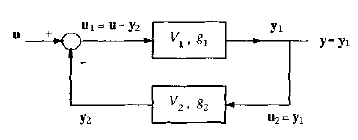
\includegraphics[width = \linewidth]{Figures/Feedback.PNG}\\
Feedback Block Combination
\begin{equation*}
\begin{aligned}
&\mathbf{y^T u} = \mathbf{y_1 ^T ( u_1 + y_2 )}\\
&= \mathbf{ y_1^T u_1 + y_1^T y_2}\\
&= \mathbf{ y_1^T u_1 + u_2^T y_2 }
\end{aligned}
\end{equation*}
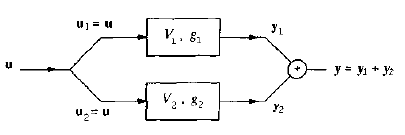
\includegraphics[width = \linewidth]{Figures/Parallel.PNG}\\
Parallel Block Combination
\begin{equation*}
\begin{aligned}
&\mathbf{y^T u} = \mathbf{(y_1  +y_2)^T u}\\
&= \mathbf{ y_1^T u + y_2^T u}\\
&= \mathbf{ y_1^T u_1 + y_2^T u_2 }
\end{aligned}
\end{equation*}
\end{column}
\end{columns}
\end{frame}


\begin{frame}
\frametitle{Positive Linear Systems}
\small
It is often possible to decompose a system into linear and nonlinear parts (Think Taylor Series Expansion). If the transfer function of the linear system is \underline{positive real}, then it has important properties that may lead to a Lyapunov function for the entire system.\\
\vspace{6pt}
Consider the $n^{th}$ order system with real coefficients in the numerator and denominator; $n \geq m$, where $n-m$ is the relative degree:
\begin{equation*}
h(s) = \frac{b_m s^m + b_{m-1}s^{m-1} + \cdots + b_0}{s^n + a_{n-1}s^{n-1} + \cdots + a_0}
\end{equation*}
\textbf{Definition:} A transfer function is \underline{Positive Real} if:
\begin{equation*}
\textrm{Re[} h(s)\text{]} \geq 0 \; \forall \; \text{Re}[s] \geq 0
\end{equation*}
It is strictly positive real if $h(s - \varepsilon)$ is positive real for some $\varepsilon >0$.
\textbf{Example: Positive Real Transfer Function}\\
\begin{equation*}
h(s) = \frac{1}{s+a}
\end{equation*}
\end{frame}

\begin{frame}
\frametitle{Positive Linear Systems}
\footnotesize
$h(s) = \frac{1}{s+a}$ is the transfer function for a first order system. With $a>0$, corresponding to the complex variable $s = \sigma + j \omega$.
\begin{equation*}
h(s) = \frac{1}{(\sigma + a) + j\omega} = \frac{\sigma + a - j\omega}{(\sigma + a)^2 + \omega^2}
\end{equation*}
Looking at the real part: $\text{Re}[h(s)] \geq 0$ if $\sigma \geq 0$. Thus $h(s)$ is a positive real function. In fact, $h(s)$ is strictly positive real. For example: by choosing $\varepsilon = a/2$.\\
\vspace{6pt}
Note that this can be difficult to perform for higher order systems.\\
\vspace{6pt}
\textbf{Theorem}: A transfer function is strictly positive real (SPR) iff
\begin{enumerate}
\item $h(s)$ is a strictly stable transfer function
\item the real part of $h(s)$ is strictly positive along the $j\omega$ axis $\forall \; \omega \geq 0, \text{Re}[h(j\omega)] >0$.
\end{enumerate}
The Necissary conditions for SPR are:
\begin{itemize}
\item $h(s)$ is strictly stable
\item Nyquist plot $h(j\omega)$ lies entirely in the right-half complex plane
\item $h(s)$ has relative degree of $0$ or $1$.
\item $h(s)$ is strictly minimum phase (all zeros in the left-half complex plane)
\end{itemize}
\end{frame}

\begin{frame}
\frametitle{Positive Linear Systems}
\small
\textbf{Examples:}
\begin{equation*}
\begin{aligned}
h_1(s) = \frac{s-1}{s^2 + as +b} \quad h_2(s) = \frac{s+1}{s^2 - s +1} \\
h_3(s) = \frac{1}{s^2 + as + b} \quad h_4(s) = \frac{s+1}{s^2 + s+ 1} \quad h_5(s) = \frac{1}{s}
\end{aligned}
\end{equation*}
\begin{enumerate}
\item $h_1(s)$ is not minimum phase since it contains a zero in the right-half complex plane. This precludes $h_1(s)$ from meeting the necessary conditions to be \textit{Strictly Positive Real}.\\
\item $h_2$ is not stable since the poles do not all lie in the left-half complex plane. $\frac{1}{2} \pm \sqrt(5)$ are the poles.
\item $h_3(s)$ has relative degree greater than 1.
\item $h_4(j \omega) = \frac{j \omega + 1}{-\omega^2 + j\omega +1} = \frac{[j \omega + 1][- \omega^2 - j \omega + 1]}{[1 - \omega^2]^2 + \omega^2}$ and $\text{Re}[h_4(j\omega)] = \frac{-\omega^2 + 1 + \omega^2}{[1 - \omega^2]^2 + \omega^2} = \frac{1}{[1 - \omega^2]^2 + \omega^2} \quad \checkmark$
\item $h_5(s) = \frac{1}{s}$ is an integrator. $h(s = \sigma + j\omega) = \frac{\sigma - j\omega}{\sigma^2 + \omega^2}$. This is positive real, but not strictly positive real.
\end{enumerate}
\end{frame}

\begin{frame}
\frametitle{Kalman-Yakubovich Lemma}
\small
A transfer function of a system in \textit{Strictly Positive Real} (SPR) if the following holds. Consider a controllable LTI system. (i.e.) the controllability matrix has full rank: 
\begin{equation*}
C = [B \;  AB \;  A^2B \;  \cdots \; A^{n-1}B]
\end{equation*}
and for the system:
\begin{equation*}
\begin{aligned}
\dot{x} &= Ax + bu\\
y &= c^T x
\end{aligned}
\end{equation*}
The transfer function $h(s) = C^T[sI - A]^{-1}b$ is strictly positive real iff:
\begin{equation*}
\exists \; P>0, \exists Q >0 \ni A^T P + P A = -Q \; \& \; Pb = c
\end{equation*}
\end{frame}


% \begin{frame}
% \frametitle{The Passivity Formalism}
% \small

% \end{frame}

% \begin{frame}
% \frametitle{Absolute Stability}
% \small

% \end{frame}

% \begin{frame}
% \frametitle{Establishing Boundedness Signals}
% \small

% \end{frame}

% \begin{frame}
% \frametitle{Existence and Unicity Solutions}
% \small

% \end{frame}

%%
%% Blank Slide
%%
% \begin{frame}
% \frametitle{}
% \end{frame}

%%
%% Dual Column Slide
%%
% \begin{frame}
% \frametitle{1st Order System - Phase Plane Example}
% \begin{columns}
% \begin{column}{0.5\textwidth}
% Text 1
% \end{column}
% \begin{column}{0.5\textwidth}
% Text 2
% \end{column}
% \end{columns}
% \end{frame}






\end{document}